\documentclass[11pt]{article}

% Change "review" to "final" to generate the final (sometimes called camera-ready) version.
% Change to "preprint" to generate a non-anonymous version with page numbers.
\usepackage{acl}

% Standard package includes
\usepackage{times}
\usepackage{latexsym}

% For proper rendering and hyphenation of words containing Latin characters (including in bib files)
\usepackage[T1]{fontenc}
% For Vietnamese characters
% \usepackage[T5]{fontenc}
% See https://www.latex-project.org/help/documentation/encguide.pdf for other character sets

% This assumes your files are encoded as UTF8
\usepackage[utf8]{inputenc}

% This is not strictly necessary, and may be commented out,
% but it will improve the layout of the manuscript,
% and will typically save some space.
\usepackage{microtype}

% This is also not strictly necessary, and may be commented out.
% However, it will improve the aesthetics of text in
% the typewriter font.
\usepackage{inconsolata}

%Including images in your LaTeX document requires adding
%additional package(s)
\usepackage{graphicx}

% If the title and author information does not fit in the area allocated, uncomment the following
%
%\setlength\titlebox{<dim>}
%
% and set <dim> to something 5cm or larger.

\usepackage{placeins}

\title{Introduction to AI and Text Analytics 2025 Group Report}

% Author information can be set in various styles:
% For several authors from the same institution:
% \author{Author 1 \and ... \and Author n \\
%         Address line \\ ... \\ Address line}
% if the names do not fit well on one line use
%         Author 1 \\ {\bf Author 2} \\ ... \\ {\bf Author n} \\
% For authors from different institutions:
% \author{Author 1 \\ Address line \\  ... \\ Address line
%         \And  ... \And
%         Author n \\ Address line \\ ... \\ Address line}
% To start a separate ``row'' of authors use \AND, as in
% \author{Author 1 \\ Address line \\  ... \\ Address line
%         \AND
%         Author 2 \\ Address line \\ ... \\ Address line \And
%         Author 3 \\ Address line \\ ... \\ Address line}

\author{
Team members (sorted by last name): \\
Weixuan Gu, Zonjin Han, Saisha Hiray, Sanya Kapoor, Chris Luckhurst, Disen Zhu
}

%\author{
%  \textbf{First Author\textsuperscript{1}},
%  \textbf{Second Author\textsuperscript{1,2}},
%  \textbf{Third T. Author\textsuperscript{1}},
%  \textbf{Fourth Author\textsuperscript{1}},
%\\
%  \textbf{Fifth Author\textsuperscript{1,2}},
%  \textbf{Sixth Author\textsuperscript{1}},
%  \textbf{Seventh Author\textsuperscript{1}},
%  \textbf{Eighth Author \textsuperscript{1,2,3,4}},
%\\
%  \textbf{Ninth Author\textsuperscript{1}},
%  \textbf{Tenth Author\textsuperscript{1}},
%  \textbf{Eleventh E. Author\textsuperscript{1,2,3,4,5}},
%  \textbf{Twelfth Author\textsuperscript{1}},
%\\
%  \textbf{Thirteenth Author\textsuperscript{3}},
%  \textbf{Fourteenth F. Author\textsuperscript{2,4}},
%  \textbf{Fifteenth Author\textsuperscript{1}},
%  \textbf{Sixteenth Author\textsuperscript{1}},
%\\
%  \textbf{Seventeenth S. Author\textsuperscript{4,5}},
%  \textbf{Eighteenth Author\textsuperscript{3,4}},
%  \textbf{Nineteenth N. Author\textsuperscript{2,5}},
%  \textbf{Twentieth Author\textsuperscript{1}}
%\\
%\\
%  \textsuperscript{1}Affiliation 1,
%  \textsuperscript{2}Affiliation 2,
%  \textsuperscript{3}Affiliation 3,
%  \textsuperscript{4}Affiliation 4,
%  \textsuperscript{5}Affiliation 5
%\\
%  \small{
%    \textbf{Correspondence:} \href{mailto:email@domain}{email@domain}
%  }
%}

\begin{document}
\maketitle
\begin{abstract}



\end{abstract}

\section{Introduction}



\section{Methods}

\subsection{Preliminary Clustering Analysis}

This preliminary clustering analysis aimed to investigate whether sentence embeddings exhibit natural groupings across participant, intervention, and outcome fields. The purpose of this stage was to evaluate whether such fields are separable in embedding space and whether this structure can inform pipeline design.

\subsubsection{Data Preparation and Label Construction}

Token-level annotations from EBM-NLP were converted into flat BIO tags (“O”, “B”, “I”), following the preprocessing steps suggested in the Task 2 course notebook~\cite{uob_task2_notebook}. Tokens were grouped into sentences using punctuation-based segmentation (``.'', ``!'', ``?''), while preserving the original annotations.

Sentence-level labels were heuristically derived: a sentence was labelled as field-related if it contained a minimum number of positive BIO tokens, otherwise as “other”. This produced three binary datasets: participants vs others, interventions vs others, and outcomes vs others. These labels are approximate, as sentences may contain multiple fields.

\subsubsection{Sentence Embeddings}

Sentences were encoded using the pretrained sentence-transformer model \texttt{all-MiniLM-L6-v2}~\cite{reimers-2019-sentence-bert} to obtain sentence embeddings.

\subsubsection{Clustering and Evaluation}

Two unsupervised methods were applied: K-means clustering ($k = 2$--$5$ for the binary tasks and $k = 3$ for the P/I/O task) and hierarchical agglomerative clustering (HAC). Clustering quality was evaluated geometrically using silhouette scores and semantically by examining the correspondence between cluster compositions and sentence-level labels. For the mixed P/I/O setting, additional cluster--label alignment metrics (ARI, NMI, and Purity) were also calculated, and silhouette sweeps were performed across multiple values of $k$.

\subsubsection{Visualisation}

The embeddings were projected into two-dimensional space using principal component analysis (PCA) and visualised using both gold labels and cluster assignments.

\subsubsection{Combined P/I/O Analysis}

A supplementary P/I/O analysis assigned each sentence to the field with the highest BIO token count, with ties labelled as \textit{mixed} and empty cases as \textit{other}. Mixed and other were excluded for three-way clustering, focusing on dominant field assignments.

\section{Experimental Evaluation}

\subsection{Preliminary Clustering Results}

\paragraph{Participants vs Other}

Participant-related clustering showed weak correspondence between clusters and labels. In K-means ($k = 2$--$5$), participant proportions remained low and similar across clusters, typically around 15\%--21\%, with a maximum of 28.7\%, indicating no participant-dominant cluster. HAC showed a comparable pattern.

\begin{figure}[htbp]
    \centering
    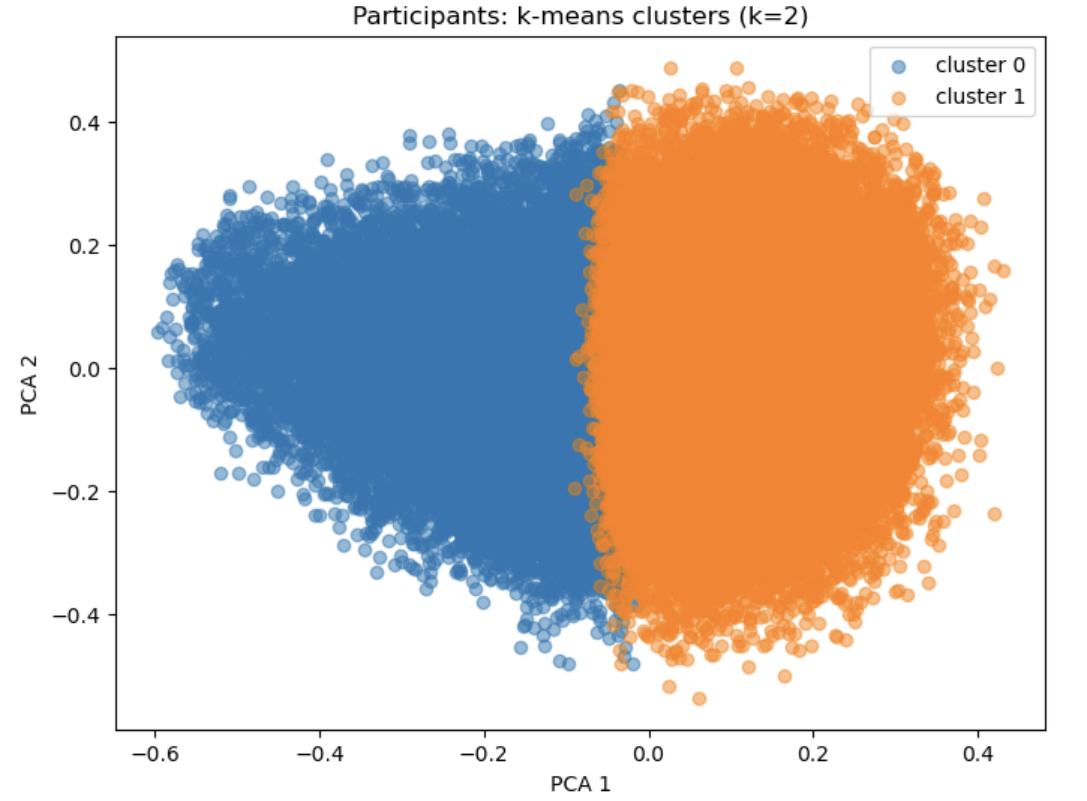
\includegraphics[width=0.5\linewidth]{figures/participants_pca.png}
    \caption{PCA projection for participant-related sentences.}
    \label{fig:participants_pca}
\end{figure}
\FloatBarrier

The PCA visualization showed an extensive overlap between the participant and the other sentences, indicating weak separability.

\paragraph{Interventions vs Other}

Intervention-related clustering showed clearer structure. K-means identified clusters with substantially higher intervention proportions, up to about 45\%, compared with about 18\%--22\% in less enriched clusters. HAC showed a similar contrast, with 36.6\% versus 18.7\% intervention-labelled sentences across clusters, suggesting consistent local enrichment.

\begin{figure}[htbp]
    \centering
    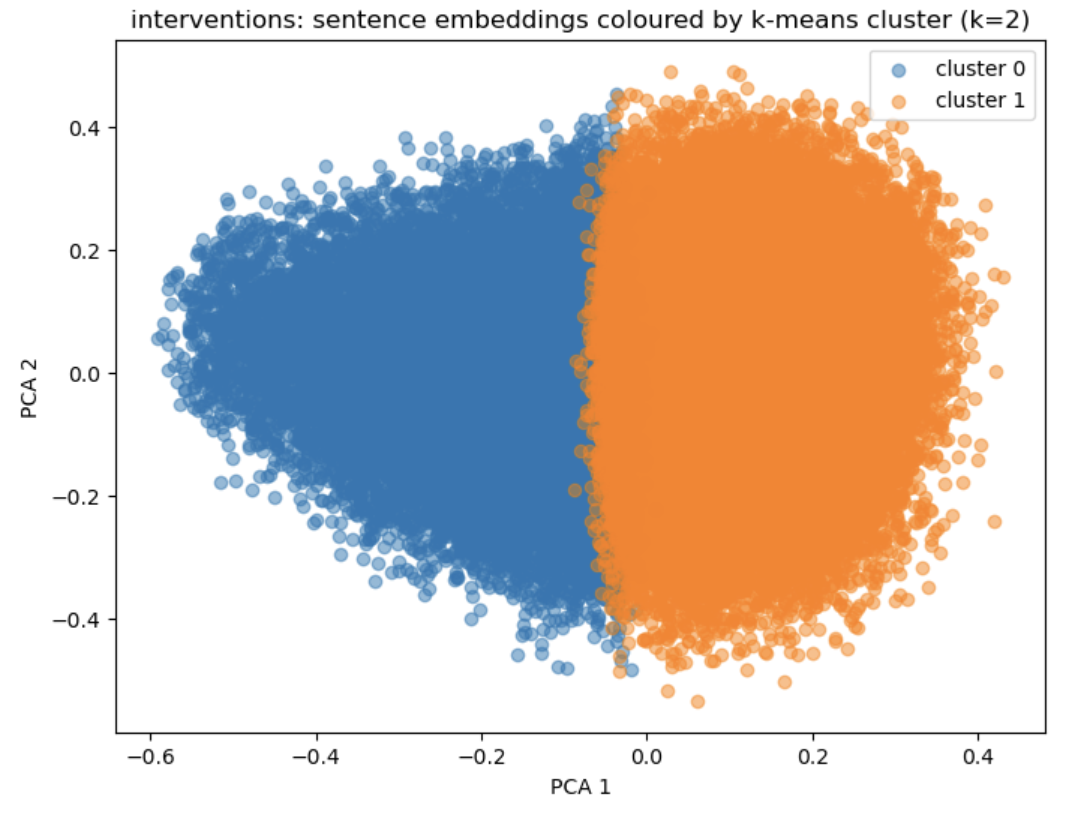
\includegraphics[width=0.5\linewidth]{figures/interventions_pca.png}
    \caption{PCA projection for intervention-related sentences.}
    \label{fig:interventions_pca}
\end{figure}

Despite overlap in PCA space, intervention-related sentences were less uniformly distributed than participant-related sentences, indicating stronger but still incomplete separability.

\paragraph{Outcomes vs Other}

Outcome-related clustering exhibited the strongest signal. K-means produced clusters with up to about 52\% outcome-labelled sentences, indicating local dominance. HAC showed smaller but consistent differences, with 39.9\% versus 35.5\%.

\begin{figure}[htbp]
    \centering
    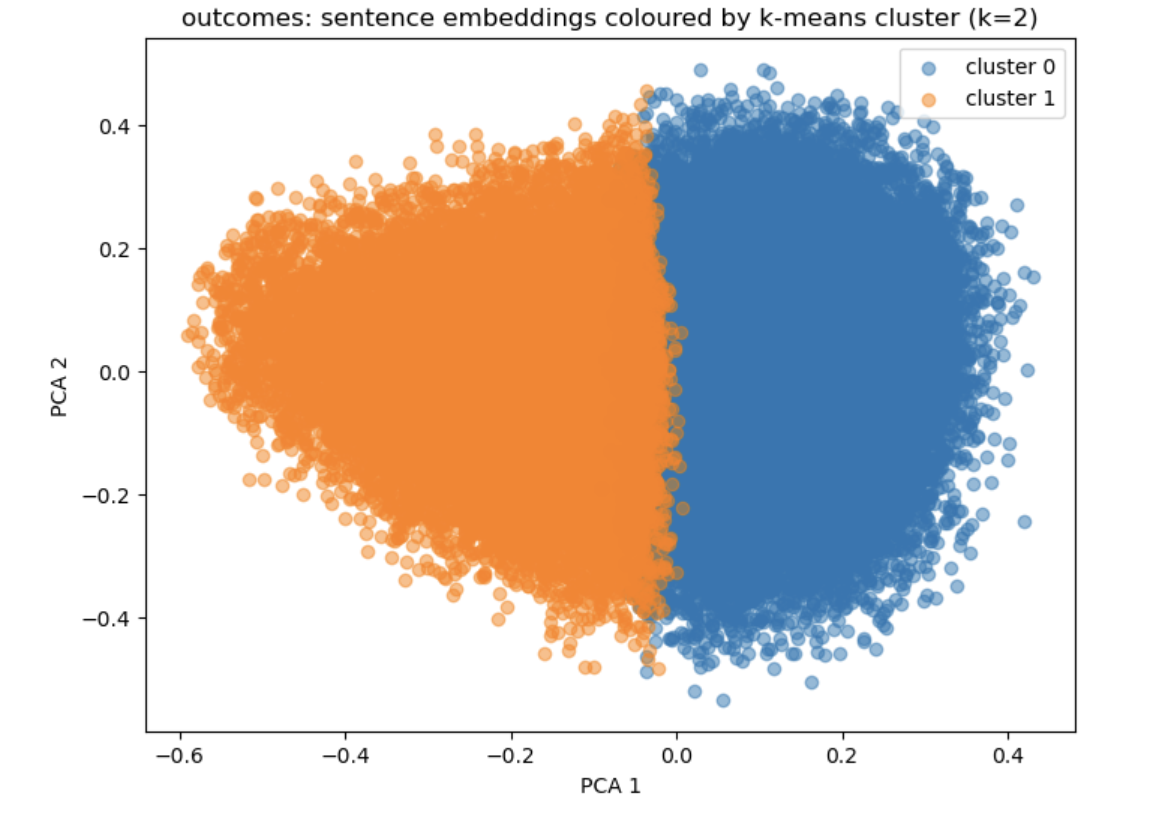
\includegraphics[width=0.5\linewidth]{figures/outcome_pca.png}
    \caption{PCA projection for outcome-related sentences.}
    \label{fig:outcomes_pca}
\end{figure}

Although PCA still showed substantial overlap, outcome-related content contributed more strongly to embedding structure than participants and, in some cases, interventions.

\subsubsection{Combined P/I/O Analysis}

Before filtering, the mixed class accounted for about 3.2\% of sentences. After excluding mixed and other, clustering was performed on dominant P/I/O labels.

\begin{figure}[htbp]
    \centering
    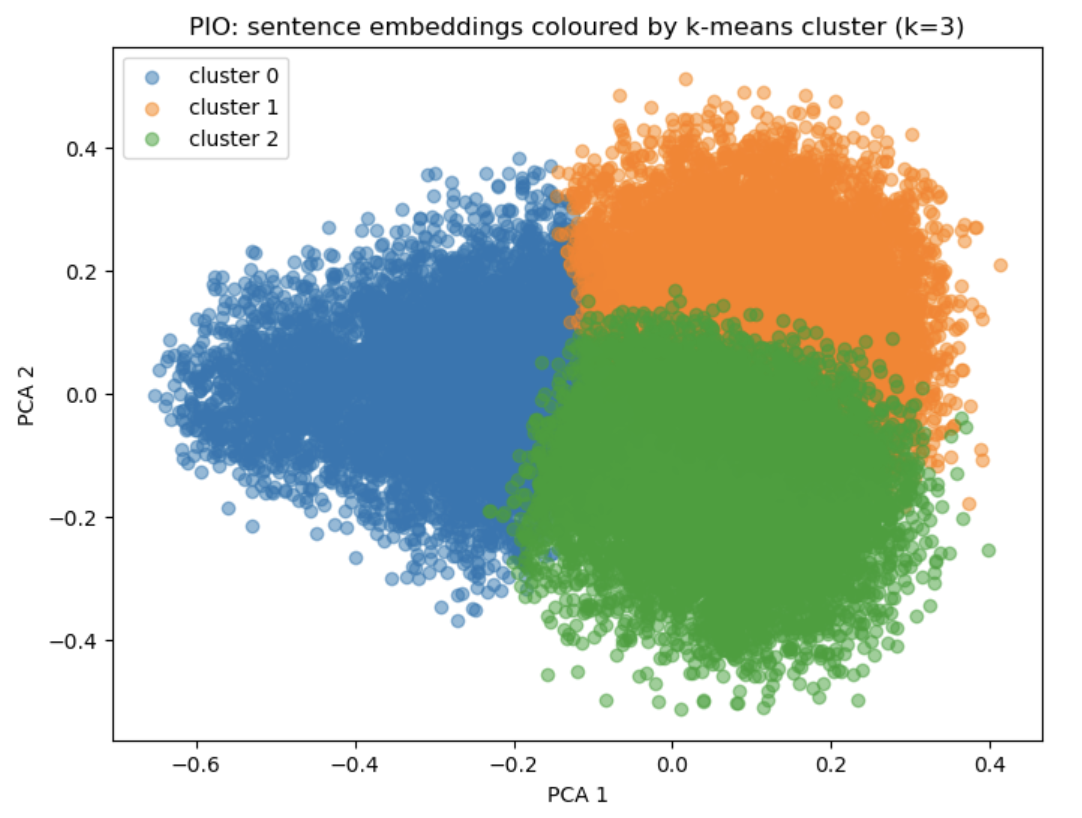
\includegraphics[width=0.5\linewidth]{figures/pio_pca.png}
    \caption{PCA projection for combined P/I/O analysis.}
    \label{fig:pio_pca}
\end{figure}

K-means ($k = 3$) produced visually distinct clusters in PCA space, but cluster compositions remained mixed, with outcomes dominating all clusters (about 47\%--58\%) and participants consistently the smallest class. HAC showed a similar pattern. The silhouette score for the three-way K-means solution was only 0.0269, reflecting weak overall geometric separation.

Cluster--label alignment metrics further confirmed this weak correspondence. For joint P/I/O K-means clustering, ARI was 0.012, NMI was 0.007, and Purity was 0.516. HAC produced similarly weak alignment (ARI = 0.005, NMI = 0.004, Purity = 0.527). A silhouette sweep across $k = 2$ to $8$ showed the highest value at $k = 2$ (0.031), with lower values from $k = 3$ onward, around 0.023--0.027. Thus, $k = 3$ remained an interpretable choice aligned with the three schema fields, but not because the embedding space naturally supported a strong three-cluster separation.

\subsubsection{Overall Interpretation}

Across all experiments, sentence embeddings exhibited spatial structure, but the correspondence between this structure and the schema fields was weak. Participants showed the weakest clustering signal, while interventions and outcomes showed stronger local enrichment, although none formed clear, field-specific clusters.

The combined P/I/O analysis also confirmed that embedding geometry does not map cleanly onto schema categories. In other words, the three-way clustering failed to separate participants, interventions, and outcomes in a meaningful way. These results show that unsupervised clustering alone is insufficient for schema extraction, motivating the use of explicit extraction pipelines.

\subsubsection{Limitations}

This analysis has several limitations. Sentence-level labels were heuristically derived from token-level annotations, and sentences may contain multiple fields, introducing noise. In addition, PCA provides only a low-dimensional approximation of the embedding space.

Although there are limitations, the results still provide useful guidance for subsequent pipeline design.

\section{Conclusions}









% Bibliography entries for the entire Anthology, followed by custom entries
%\bibliography{anthology,custom}
% Custom bibliography entries only
\bibliography{custom}

\appendix

\section{Example Appendix}
\label{sec:appendix}

This is an appendix.

\end{document}
